\documentclass{ltxdoc}
\title{Commutative LBC Actions Proposal}

\usepackage{amsmath}  % extended mathematics
\usepackage{units}    % non-stacked fractions and better unit spacing
\usepackage{fancyvrb} % extended verbatim environments
\usepackage{tikz}
\usepackage{tkz-berge}
\usepackage{mathtools}
\usepackage{forest}
\usetikzlibrary{arrows.meta,chains, decorations.pathreplacing, shapes.multipart}

\begin{document}

%\forestset{
  %default preamble={
    %for tree={circle,draw}
  %}
%}

\section{Concrete}

\vspace{30px}

\[ \sigma_0 T_0^1 \sigma_1 \]

\vspace{30px}

\[ \Sigma \]

\vspace{30px}

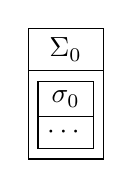
\begin{tikzpicture}[
   double/.style={draw, anchor=text, rectangle split,rectangle split parts=2}
  ]

  \node[double] {$\Sigma_0$
    \nodepart{second}
      \tikz{\node[double]{$\sigma_0$ \nodepart{second} $\cdots$ }}
  };

\end{tikzpicture}

\vspace{30px}

\[ \Sigma_0 \]

\vspace{30px}

\[ \Rightarrow \! \! \Sigma_0 \]

\vspace{30px}

\[ \sigma_0 \implies \sigma_1 \]

\vspace{30px}

\begin{align*}
  \sigma_0 + T_0^1 &= \sigma_1 \\
  \sigma_1 + T_1^2 &= \sigma_2 \\
  \sigma_2 + T_2^3 &= \sigma_3
\end{align*}

\vspace{30px}

\begin{forest}
% TODO: Draw the rectangles
  [$\sigma_0$,
    [$T_0^1$ [$\sigma_1$ [$T_1^2$ [$\sigma_2$]]]]]
\end{forest}

\vspace{30px}

\begin{forest}
  [,phantom
    [$\Rightarrow \! \! \Sigma_0$,tier=top,name=b0,calign=first]
    [$\Rightarrow \! \! \Sigma_1$,tier=top,name=b1,fit=rectangle
     [$\sigma_0 \implies \sigma_4$,edge=dashed
       [$\sigma_0 \implies \sigma_2$
         [$\sigma_0 \implies \sigma_1$ [$\sigma_0 \; T_0^1 \; \sigma_1$,magenta ] ]
         [$\sigma_1 \implies \sigma_2$ [$\sigma_1 \; T_1^2 \; \sigma_2$,magenta ] ]
       ]
       [$\sigma_2 \implies \sigma_4$
         [$\sigma_2 \implies \sigma_3$ [$\sigma_2 \; T_2^3 \; \sigma_3$,magenta ] ]
         [$\sigma_3 \implies \sigma_4$ [$\sigma_3 \; T_3^4 \; \sigma_4$,magenta ] ]
       ]
     ]
    ]
  ]
  \draw[->] (b0) to[out=east,in=west] (b1);
\end{forest}

\vspace{30px}

\section{Merging}

\vspace{30px}

%\begin{forest}

% TODO: Show single s0 -> s2
% TODO: Show s0 -> s3 both ways (associativity)

%\end{forest}


\vspace{30px}

\section{Serial}

\vspace{30px}

\begin{forest}
  [,phantom
    [$\Rightarrow \! \! \Sigma_0$,tier=top,name=b0,calign=first]
    [,circle,draw,tier=top,name=s01,fit=rectangle
      [$\sigma_0 \implies \sigma_1$,edge=dashed [$\sigma_0 \; T_0^1 \; \sigma_1$,magenta] ]
    ]
    [,circle,draw,tier=top,name=s02
      [$\sigma_0 \implies \sigma_2$,edge=dashed,name=i02 [$\sigma_1 \; T_1^2 \; \sigma_2$,magenta,name=i12] ]
    ]
    [,circle,draw,tier=top,name=s03
      [$\sigma_0 \implies \sigma_3$,edge=dashed,name=i03 [$\sigma_2 \; T_2^3 \; \sigma_3$,magenta,name=i23] ]
    ]
    [$\Rightarrow \! \! \Sigma_1$,tier=top,name=b1,fit=rectangle
      [$\sigma_0 \implies \sigma_4$,edge=dashed,name=i04 [$\sigma_3 \; T_3^4 \; \sigma_4$,magenta,name=i34] ]
    ]
  ]
  \draw[->] (b0) to[out=south,in=west] (s01);
  \draw[->] (s01) to[out=east,in=west] (s02);
  \draw[->] (s02) to[out=east,in=west] (s03);
  \draw[->] (s03) to[out=east,in=north] (b1);
  \draw[dashed,->] (s01) to[out=east,in=north west] (i12);
  \draw[dashed,->] (s02) to[out=east,in=north west] (i23);
  \draw[dashed,->] (s03) to[out=east,in=north west] (i34);
\end{forest}


\vspace{30px}

\section{Pre-naive}

\vspace{30px}

\[ D_1 \coloneqq \; \; \sigma_0 T_0^1 \sigma_1 \]

\vspace{30px}

\[ M_{12} \coloneqq \; \; \sigma_1 \implies \sigma_2 \]

\vspace{30px}

\[ A_1 \coloneqq \; \; \Rightarrow \! \! \Sigma_1 \]

\vspace{30px}

\[ ((((A + D_1) + D_2) + D_3) + D_4) \]

\vspace{30px}

\section{Naive}

\vspace{30px}

Data

\vspace{30px}

\begin{forest}
 [,phantom
   [,phantom
     [,phantom
       [,phantom [$D_1$] ]
       [,phantom [$D_2$] ]
     ]
     [,phantom
       [,phantom [$D_3$] ]
       [,phantom [$D_4$] ]
     ]
   ]
   [,phantom
     [,phantom
       [,phantom [$D_5$] ]
       [,phantom [$D_6$] ]
     ]
     [,phantom
       [,phantom [$D_7$] ]
       [,phantom [$D_8$] ]
     ]
   ]
 ]
\end{forest}

\vspace{30px}

Base proofs

\vspace{30px}

\begin{forest}
 [,phantom
   [,phantom
     [,phantom
       [$B_1$ [$D_1$] ]
       [$B_2$ [$D_2$] ]
     ]
     [,phantom
       [$B_3$ [$D_3$] ]
       [$B_4$ [$D_4$] ]
     ]
   ]
   [,phantom
     [,phantom
       [$B_5$ [$D_5$] ]
       [$B_6$ [$D_6$] ]
     ]
     [,phantom
       [$B_7$ [$D_7$] ]
       [$B_8$ [$D_8$] ]
     ]
   ]
 ]
\end{forest}

\vspace{30px}

Merge proofs

\vspace{30px}

\begin{forest}
 [,phantom
   [,phantom
     [$M_{12}$
       [$B_1$ [$D_1$] ]
       [$B_2$ [$D_2$] ]
     ]
     [$M_{34}$
       [$B_3$ [$D_3$] ]
       [$B_4$ [$D_4$] ]
     ]
   ]
   [,phantom
     [$M_{56}$
       [$B_5$ [$D_5$] ]
       [$B_6$ [$D_6$] ]
     ]
     [$M_{78}$
       [$B_7$ [$D_7$] ]
       [$B_8$ [$D_8$] ]
     ]
   ]
 ]
\end{forest}

\vspace{30px}

All the way

\vspace{30px}

\begin{forest}
 [,phantom
   [$M_{1-4}$
     [$M_{12}$
       [$B_1$ [$D_1$] ]
       [$B_2$ [$D_2$] ]
     ]
     [$M_{34}$
       [$B_3$ [$D_3$] ]
       [$B_4$ [$D_4$] ]
     ]
   ]
   [$M_{5-8}$
     [$M_{56}$
       [$B_5$ [$D_5$] ]
       [$B_6$ [$D_6$] ]
     ]
     [$M_{78}$
       [$B_7$ [$D_7$] ]
       [$B_8$ [$D_8$] ]
     ]
   ]
 ]
\end{forest}

\vspace{30px}

\begin{forest}
  [,phantom
    [$A_0$,tier=top,name=b0,calign=first]
    [$A_1$,tier=top,name=b1,fit=rectangle
     [$M_{1-8}$,edge=dotted
       [$M_{1-4}$
         [$M_{12}$
           [$B_1$ [$D_1$] ]
           [$B_2$ [$D_2$] ]
         ]
         [$M_{34}$
           [$B_3$ [$D_3$] ]
           [$B_4$ [$D_4$] ]
         ]
       ]
       [$M_{5-8}$
         [$M_{56}$
           [$B_5$ [$D_5$] ]
           [$B_6$ [$D_6$] ]
         ]
         [$M_{78}$
           [$B_7$ [$D_7$] ]
           [$B_8$ [$D_8$] ]
         ]
       ]
     ]
    ]
  ]
  \draw[->] (b0) to[out=east,in=west] (b1);
\end{forest}

\vspace{30px}

\section{Better Solution}

\vspace{30px}

I wish we could lay horizontal?

A

\vspace{30px}

\begin{forest}
   [,phantom
     [,phantom
       [,phantom [$D_1$,green!50!black] ]
       [,phantom [$D_2$,green!50!black] ]
     ]
     [,phantom
       [,phantom [$D_3$,green!50!black] ]
       [,phantom [$D_4$,green!50!black] ]
     ]
   ]
\end{forest}

\vspace{30px}

B

\vspace{30px}

\begin{forest}
  [,phantom
   [,phantom,tier=top,name=b0,calign=first]
   [,phantom,tier=top,name=b1,fit=rectangle
      [,phantom
       [,phantom
         [$B_1$,green!50!black [$D_1$,green!50!black] ]
         [$B_2$,green!50!black [$D_2$,green!50!black] ]
       ]
       [,phantom
         [$B_3$,green!50!black [$D_3$,green!50!black] ]
         [$B_4$,green!50!black [$D_4$,green!50!black] ]
       ]
     ]
   ]
   [,phantom,tier=top,name=b2
     [,phantom
       [,phantom
         [,phantom [$D_5$,purple!80!black] ]
         [,phantom [$D_6$,purple!80!black] ]
       ]
       [,phantom
         [,phantom [,phantom] ]
         [,phantom [,phantom] ]
       ]
     ]
   ]
  ]
\end{forest}

\vspace{30px}

C

\vspace{30px}

\begin{forest}
  [,phantom
   [,phantom,tier=top,name=b0,calign=first]
   [,phantom,tier=top,name=b1,fit=rectangle
     [,phantom
       [$M_{12}$,green!50!black
         [$B_1$,green!50!black [$D_1$,green!50!black] ]
         [$B_2$,green!50!black [$D_2$,green!50!black] ]
       ]
       [$M_{34}$,green!50!black
         [$B_3$,green!50!black [$D_3$,green!50!black] ]
         [$B_4$,green!50!black [$D_4$,green!50!black] ]
       ]
     ]
   ]
   [,phantom,tier=top,name=b2
     [,phantom
       [,phantom
         [$B_5$,purple!80!black [$D_5$,purple!80!black] ]
         [$B_6$,purple!80!black [$D_6$,purple!80!black] ]
       ]
       [,phantom
         [,phantom [$D_7$,purple!80!black] ]
         [,phantom [$D_8$,purple!80!black] ]
       ]
     ]
   ]
  ]
\end{forest}

\vspace{30px}

D

\vspace{30px}

\begin{forest}
  [,phantom
    [$A_0$,tier=top,name=b0,calign=first]
    [$A_1$,tier=top,name=b1,fit=rectangle
     [$M_{1-4}$,green!50!black,edge=dotted
       [$M_{12}$,green!50!black
         [$B_1$,green!50!black [$D_1$,green!50!black] ]
         [$B_2$,green!50!black [$D_2$,green!50!black] ]
       ]
       [$M_{34}$,green!50!black
         [$B_3$,green!50!black [$D_3$,green!50!black] ]
         [$B_4$,green!50!black [$D_4$,green!50!black] ]
       ]
     ]
    ]
   [,phantom,tier=top,name=b2
     [,phantom
       [$M_{56}$,purple!80!black
         [$B_5$,purple!80!black [$D_5$,purple!80!black] ]
         [$B_6$,purple!80!black [$D_6$,purple!80!black] ]
       ]
       [,phantom
         [$B_7$,purple!80!black [$D_7$,purple!80!black] ]
         [$B_8$,purple!80!black [$D_8$,purple!80!black] ]
       ]
     ]
   ]
   [,phantom,tier=top,name=b3
     [,phantom
       [,phantom
         [,phantom [$D_9$,yellow!60!black] ]
         [,phantom [$D_{10}$,yellow!60!black] ]
       ]
       [,phantom
         [,phantom [,phantom] ]
         [,phantom [,phantom] ]
       ]
     ]
   ]
  ]
  \draw[->] (b0) to[out=east,in=west] (b1);
\end{forest}

\vspace{30px}

E

\vspace{30px}

\begin{forest}
  [,phantom
    [$A_1$,tier=top,name=b1,calign=first]
    [,phantom,tier=top,name=b2,fit=rectangle
     [,phantom
       [$M_{56}$,purple!80!black
         [$B_5$,purple!80!black [$D_5$,purple!80!black] ]
         [$B_6$,purple!80!black [$D_6$,purple!80!black] ]
       ]
       [$M_{78}$,purple!80!black
         [$B_7$,purple!80!black [$D_7$,purple!80!black] ]
         [$B_8$,purple!80!black [$D_8$,purple!80!black] ]
       ]
     ]
    ]
    [,phantom,tier=top,name=b3
     [,phantom
       [,phantom
         [$B_9$,yellow!60!black [$D_9$,yellow!60!black] ]
         [$B_{10}$,yellow!60!black [$D_{10}$,yellow!60!black] ]
       ]
       [,phantom
         [,phantom [$D_{11}$,yellow!60!black] ]
         [,phantom [$D_{12}$,yellow!60!black] ]
       ]
     ]
    ]
  ]
\end{forest}

\vspace{30px}

F

\vspace{30px}

\begin{forest}
  [,phantom
    [$A_1$,tier=top,name=b1,calign=first]
    [$A_2$,tier=top,name=b2,fit=rectangle
     [$M_{5-8}$,purple!80!black,edge=dotted
       [$M_{56}$,purple!80!black
         [$B_5$,purple!80!black [$D_5$,purple!80!black] ]
         [$B_6$,purple!80!black [$D_6$,purple!80!black] ]
       ]
       [$M_{78}$,purple!80!black
         [$B_7$,purple!80!black [$D_7$,purple!80!black] ]
         [$B_8$,purple!80!black [$D_8$,purple!80!black] ]
       ]
     ]
    ]
    [,phantom,tier=top,name=b3
     [,phantom
       [$M_{9-10}$,yellow!60!black
         [$B_9$,yellow!60!black [$D_9$,yellow!60!black] ]
         [$B_{10}$,yellow!60!black [$D_{10}$,yellow!60!black] ]
       ]
       [,phantom
         [$B_{11}$,yellow!60!black [$D_{11}$,yellow!60!black] ]
         [$B_{12}$,yellow!60!black [$D_{12}$,yellow!60!black] ]
       ]
     ]
    ]
    [,phantom,tier=top,name=b4
     [,phantom
       [,phantom
         [,phantom [$D_{13}$,blue!80!black] ]
         [,phantom [$D_{14}$,blue!80!black] ]
       ]
       [,phantom
         [,phantom [,phantom] ]
         [,phantom [,phantom] ]
       ]
     ]
    ]
  ]
  \draw[->] (b1) to[out=east,in=west] (b2);
\end{forest}

\vspace{30px}

G

\vspace{30px}

\begin{forest}
  [,phantom
    [$A_2$,tier=top,name=b2,calign=first]
    [,phantom,tier=top,name=b3,fit=rectangle
     [,phantom
       [$M_{9-10}$,yellow!60!black
         [$B_9$,yellow!60!black [$D_9$,yellow!60!black] ]
         [$B_{10}$,yellow!60!black [$D_{10}$,yellow!60!black] ]
       ]
       [$M_{11-12}$,yellow!60!black
         [$B_{11}$,yellow!60!black [$D_{11}$,yellow!60!black] ]
         [$B_{12}$,yellow!60!black [$D_{12}$,yellow!60!black] ]
       ]
     ]
    ]
    [,phantom,tier=top,name=b4
     [,phantom
       [,phantom
         [$B_{13}$,blue!80!black [$D_{13}$,blue!80!black] ]
         [$B_{14}$,blue!80!black [$D_{14}$,blue!80!black] ]
       ]
       [,phantom
         [,phantom [$D_{15}$,blue!80!black] ]
         [,phantom [$D_{16}$,blue!80!black] ]
       ]
     ]
    ]
  ]
\end{forest}

\vspace{30px}

H

\vspace{30px}

\begin{forest}
  [,phantom
    [$A_2$,tier=top,name=b2,calign=first]
    [$A_3$,tier=top,name=b3,fit=rectangle
     [$M_{9-12}$,edge=dotted, for tree={yellow!60!black}
       [$M_{9-10}$
         [$B_9$ [$D_9$] ]
         [$B_{10}$ [$D_{10}$] ]
       ]
       [$M_{11-12}$
         [$B_{11}$ [$D_{11}$] ]
         [$B_{12}$ [$D_{12}$] ]
       ]
     ]
    ]
    [,phantom,tier=top,name=b4
      [,phantom
       [$M_{13-14}$,blue!80!black
         [$B_{13}$,blue!80!black [$D_{13}$,blue!80!black] ]
         [$B_{14}$,blue!80!black [$D_{14}$,blue!80!black] ]
       ]
       [,phantom
         [$B_{15}$,blue!80!black [$D_{15}$,blue!80!black] ]
         [$B_{16}$,blue!80!black [$D_{16}$,blue!80!black] ]
       ]
      ]
    ]
    [,phantom,tier=top,name=b5
      [,phantom
        [,phantom
          [,phantom [$D_{17}$,green!50!black] ]
          [,phantom [$D_{18}$,green!50!black] ]
        ]
        [,phantom
          [,phantom [,phantom] ]
          [,phantom [,phantom] ]
        ]
      ]
    ]
 ]
  \draw[->] (b2) to[out=east,in=west] (b3);
\end{forest}

\vspace{30px}

\section{Space Waste}

\vspace{30px}

\begin{forest}
  [,phantom
    [$A_2$,tier=top,name=b2,calign=first]
    [$A_3$,tier=top,name=b3,fit=rectangle
     [$M_{9-12}$,for descendants={red}
       [$M_{9-10}$
         [$B_9$ [$D_9$] ]
         [$B_{10}$ [$D_{10}$] ]
       ]
       [$M_{11-12}$
         [$B_{11}$ [$D_{11}$] ]
         [$B_{12}$ [$D_{12}$] ]
       ]
     ]
    ]
    [,phantom,tier=top,name=b4
     [,phantom
       [$M_{13-14}$,for descendants={red}
         [$B_{13}$ [$D_{13}$] ]
         [$B_{14}$ [$D_{14}$] ]
       ]
       [,phantom
         [$B_{15}$ [$D_{15}$,red] ]
         [$B_{16}$ [$D_{16}$,red] ]
       ]
     ]
    ]
    [,phantom,tier=top,name=b5
     [,phantom
       [,phantom
         [,phantom [$D_{17}$] ]
         [,phantom [$D_{18}$] ]
       ]
       [,phantom
         [,phantom [,phantom] ]
         [,phantom [,phantom] ]
       ]
     ]
    ]
  ]
  \draw[->] (b2) to[out=east,in=west] (b3);
\end{forest}

\vspace{30px}

Compress it

\vspace{30px}

\begin{forest}
  [,phantom
    [$A_2$,tier=top,name=b2,calign=first]
    [$A_3$,tier=top,name=b3,fit=rectangle
     [$M_{9-12}$
       [$M_{13-14}$
         [,circle,draw [$D_{17}$] ]
         [,circle,draw [$D_{18}$] ]
       ]
       [,circle,draw
         [$B_{15}$ [,circle,draw ] ]
         [$B_{16}$ [,circle,draw ] ]
       ]
     ]
    ]
  ]
  \draw[->] (b2) to[out=east,in=west] (b3);
\end{forest}

\vspace{30px}

Step 2

\vspace{30px}

\begin{forest}
  [,phantom
    [$A_3$,tier=top,name=b2,calign=first]
    [,phantom,tier=top,name=b3,fit=rectangle
     [,circle,draw
       [,circle,draw
         [$B_{17}$ [,circle,draw ] ]
         [$B_{18}$ [,circle,draw ] ]
       ]
       [$M_{15-16}$
         [,circle,draw [$D_{19}$ ] ]
         [,circle,draw [$D_{20}$ ] ]
       ]
     ]
    ]
  ]
\end{forest}

\vspace{30px}

\section{Instantiation}

\vspace{30px}

\begin{forest}
  [,phantom
    [$\Rightarrow \! \! \Sigma_0$,tier=top,name=b0,calign=first]
    [$\Rightarrow \! \! \Sigma_1$,tier=top,name=b1,fit=rectangle
     [$\sigma_0 \implies \sigma_4$
       [$\sigma_4 \implies \sigma_6$
         [,circle,draw [$\sigma_8 \; T_8^9 \; \sigma_9$,magenta] ]
         [,circle,draw [$\sigma_9 \; T_9^{10} \; \sigma_{10}$,magenta] ]
       ]
       [,circle,draw
         [$\sigma_6 \implies \sigma_7$ [,circle,draw] ]
         [$\sigma_7 \implies \sigma_8$ [,circle,draw] ]
       ]
     ]
    ]
  ]
  \draw[->] (b0) to[out=east,in=west] (b1);
\end{forest}

\vspace{30px}

\begin{forest}
  [$M(M_{13-14}; M_{15-16})$
     [$M(B_{17}; B_{18})$
       [$B(\cdot)$ ]
       [$B(\cdot)$ ]
     ]
     [$M(\cdot;\cdot)$
       [$B(D_{19})$  ]
       [$B(D_{20})$  ]
     ]
   ]
\end{forest}

\vspace{30px}

\section{Succinct}

\vspace{30px}

% https://tex.stackexchange.com/questions/245251/proportional-boxes-in-tikz-array-diagram
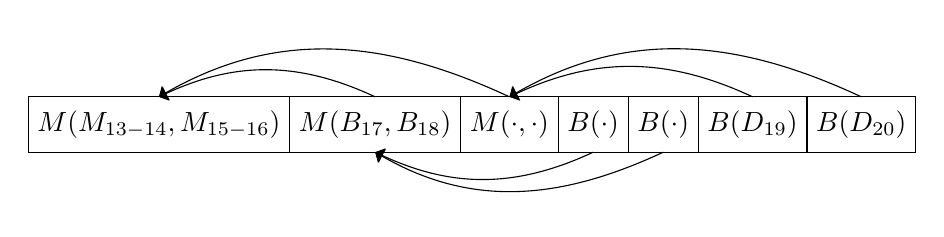
\begin{tikzpicture}[
%  -{Stealth[length = 2.5pt]},
       start chain = going right,
     node distance = 0pt,
MyStyle/.style={draw, minimum width=2em, minimum height=2em, 
                outer sep=0pt, on chain},
  ]
\node [MyStyle] (1) {$M(M_{13-14},M_{15-16})$};
\node [MyStyle] (2) {$M(B_{17},B_{18})$};
\node [MyStyle] (3) {$M(\cdot,\cdot)$};
\node [MyStyle] (4) {$B(\cdot)$};
\node [MyStyle] (5) {$B(\cdot)$};
\node [MyStyle] (6) {$B(D_{19})$};
\node [MyStyle] (7) {$B(D_{20})$};
\begin{scope}[-{Stealth[length = 2.5pt]}]
  \draw[arrows={-Triangle[angle=90:4pt]}] (2.north) [out=155, in=25] to (1.north);
  \draw[arrows={-Triangle[angle=90:4pt]}] (3.north) [out=155, in=30] to (1.north);
  \draw[arrows={-Triangle[angle=90:4pt]}] (4.south) [out=-155, in=-25] to (2.south);
  \draw[arrows={-Triangle[angle=90:4pt]}] (5.south) [out=-155, in=-30] to (2.south);
  \draw[arrows={-Triangle[angle=90:4pt]}] (6.north) [out=155, in=25] to (3.north);
  \draw[arrows={-Triangle[angle=90:4pt]}] (7.north) [out=155, in=30] to (3.north);
\end{scope}
%\draw[decorate,decoration={brace, amplitude=10pt, raise=5pt, mirror}]
%  (2.south west) to node[black,midway,below= 15pt] {$k$-elements} (7.south east);
\end{tikzpicture}


\end{document}
